\section{Introduction to Retrieval models}
\begin{itemize}
	\item Mathematical framework for defining query-document matching
\end{itemize}
\subsection{Query Analysis}
\begin{figure}[h!]
	\centering
	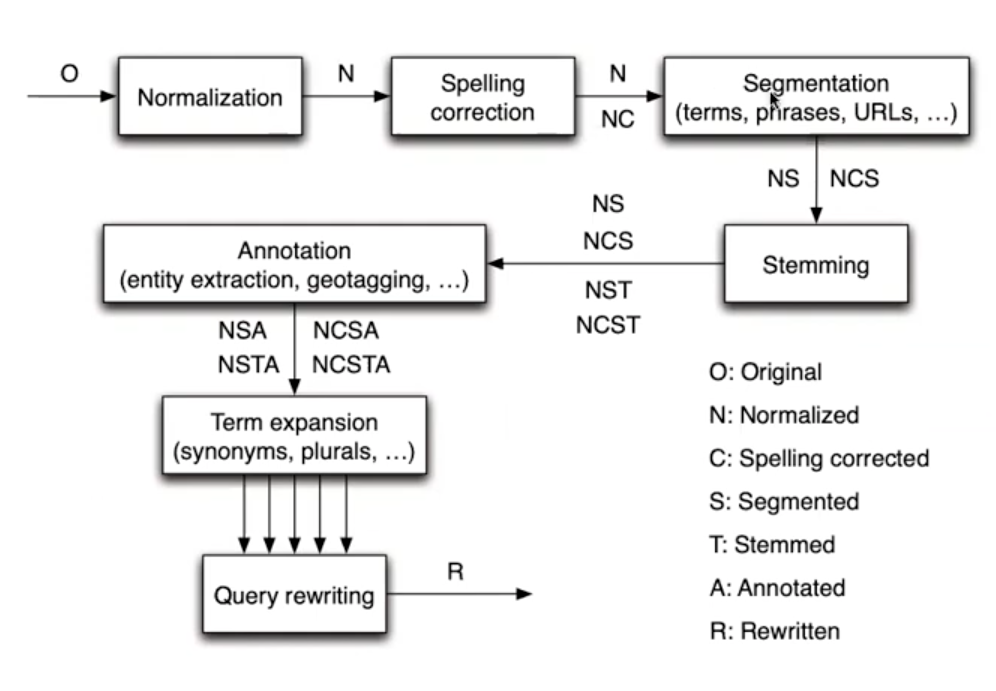
\includegraphics[width=0.5\textwidth]{figures/query_analysis_pipeline.png}
	\caption{Query analysis pipeline}
	\label{img:query_analysis_pipeline}
\end{figure}
Query analysis pipeline is given in Fig. \ref{img:query_analysis_pipeline}.
\subsection{Query Processing}
\begin{figure}[h!]
	\centering
	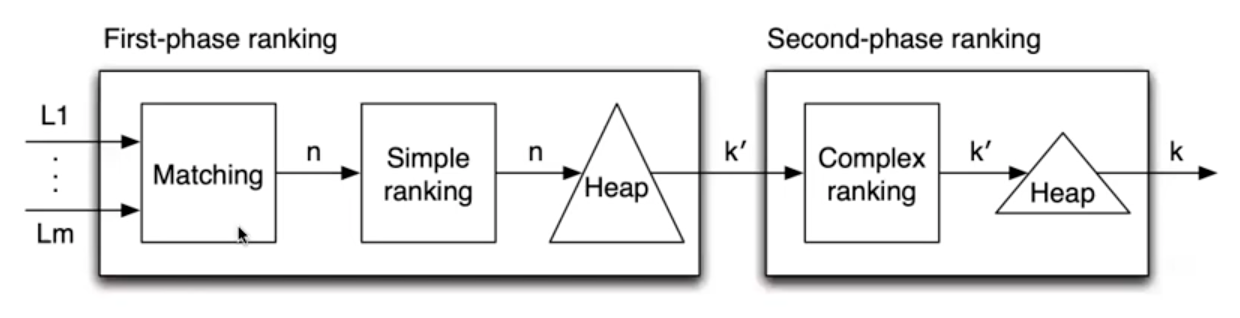
\includegraphics[width=0.5\textwidth]{figures/query_processing.png}
	\caption{Query processing}
	\label{img:query_processing}
\end{figure}
\begin{itemize}
	\item Process depicted in Fig. \ref{img:query_processing}
	\item Matching: select documents that have something to do with query
	\item Simple ranking: retrieve first ranking for a large number of documents
	\item Complex ranking: re-rank only top-k documents from simple ranking (simple ranking is fast and cheap whereas complex ranking is slow and expensive)
\end{itemize}
How to select documents?
\begin{itemize}
	\item Term-at-a-time: preprocess terms $\rightarrow$ for each term, go through inverted list of documents (and weights) $\rightarrow$ add weights of corresponding documents across terms (advantages: only one list at a time to process, disadvantages: store complete list of weights in memory)
	\item Process all inverted lists at the same time $\rightarrow$ like merge sort where you keep pointers in each list and have those pointers at the same document ids all the time (note that inverted lists have to be ordered)
	\item In practice: for websearch select documents where ALL query terms appear in documents; in cases where you want to retrieve many possible matches, select documents where at least one term from query appear (e.g. medical search)
	\item A document score is usually computed as linear combination of query-dependent and query-independent scores
\end{itemize}
\subsection{TF-IDF}
\begin{itemize}
	\item In a vector space model, documents and queries are represented in vector space
	\item Axes are mostly terms/vocabulary so that a document or query is represented by terms they contain (binary) or their frequency
	\item We can rank documents based on their cosine similarity with the query:
	$$\text{score}(d,q) = \frac{\vec{q} \cdot \vec{d}}{||\vec{q}||\cdot ||\vec{d}||}$$
	\item Documents can be therefore represented as non-negative vector of term weights (raw frequency in doc):
	\begin{figure}[ht]
		\centering
		\includegraphics[width=0.5\textwidth]{figures/language_models_tf_example.png}
		\label{img:language_models_tf_example}
	\end{figure}
	\item However, the problem here is that terms with a higher frequency in documents are automatically more important, although this is not always the case (e.g. "the"). Thus, for identifying the important terms, we can report document frequency (no. of docs in which terms occurs):
	$$\text{df}(t) \coloneqq \#\left\{d:\text{tf}(t;d)>0\right\}$$
	\item We can translate document frequencies to term weights by inverting them (inverted document frequency - \textit{IDF}):
	$$\text{idf}(t) = \log \frac{n}{\text{df}(t)} = \log n - \log \text{df}(t)$$
	The log is applied to dampen the effect of IDF.
	\item Also the term frequencies should be dampened by a monotonic, sub-linear transformation as a term occurring twice as often doesn't imply that the document is also twice as important/relevant. Together, we can define the tf-idf weights as follows:
	$$\text{tf-idf}(t;d) = \log \left(1+\text{tf}(t;d)\right) \log \frac{n}{\text{df}(t)}$$
	\item Scores are normalized by euclidean distance of document. Alternatively, we could also apply tf-idf on the relative term frequencies.
\end{itemize}
\subsection{BM25}
\begin{itemize}
	\item Probabilistic retrieval framework that extends the idea of tf-idf
	\item Instead of the log, we use a different damping functions which are easier to control:
	$$w_t = \frac{(k_1 + 1)\cdot \text{tf}(d;t)}{k_1 + \text{tf}(d;t)}\cdot \text{idf}(t)$$
	\item In addition, we normalize the term frequency by the document length: $\text{tf}'(d;t) = \text{tf}(d;t) \cdot l_{avg}/l_{d}$ ($l_{avg}$ is the average document length of collection). By this we prevent copies of documents concatenated with each other being higher rated. Putting this into our original function, we get:
	$$w_t = \frac{(k_1 + 1) \cdot \text{tf}(d;t)}{k_1 \cdot (l_d / l_{avg})+ \text{tf}(d;t)}\cdot \text{idf}(t)$$
	\item However, longer documents also tend to contain more information. Thus, we introduce another parameter $b$ that controls the normalization:
	$$w_t = \frac{(k_1 + 1) \cdot \text{tf}(d;t)}{k_1 \cdot ((1-b) + b\cdot (l_d / l_{avg}))+ \text{tf}(d;t)}\cdot \text{idf}(t)$$
	\item For very long queries, we also need to consider this normalization which can be done by multiplying another term $\frac{(k_3 + 1)\cdot \text{tf}(q;t)}{k_3 \cdot \text{tf}(q;t)}$
	\item In conclusion, the BM25 score is calculated as follows:
	$$\text{BM25} = \sum\limits_{\text{unique\hspace{1mm}} t\in q} \frac{(k_1 + 1) \cdot \text{tf}(d;t)}{k_1 \cdot ((1-b) + b\cdot (l_d / l_{avg}))+ \text{tf}(d;t)} \cdot \frac{(k_3 + 1)\cdot \text{tf}(q;t)}{k_3 + \text{tf}(q;t)} \cdot \text{idf}(t)$$
	\item Parameters $k_1$, $b$ and $k_3$ are tuned. Common defaults are $k_1 = 1.5$ and $b=0.75$
	\item It is the most widely used ranking in IR but only loosely inspired by probabilistic models
	\item Parameters:
	\begin{itemize}
		\item $k_1 \rightarrow 0 \Rightarrow$ Sum of idf
		\item $k_1 \rightarrow \infty \Rightarrow$ Sum of tf-idf
		\item b is parameter controlling the document length, if $b=0 \Rightarrow$ no normalization by document length $\Rightarrow$ not fair against short documents
		\item if $tf \rightarrow \infty \Rightarrow$ reduces to sum of idf with constant multiplication ($k_1 + 1$)
		\item long queries: cancel out with large term frequency in query
	\end{itemize}
\end{itemize}
\subsection{Statistical Language Models}
\begin{itemize}
	\item Statistical language models are a probability distribution over word sequences $P(w_1, ..., w_m)$ with which documents and queries can be represented (and uncertainty quantified)
	\item Thus, a language model describes the probability of e.g. $q$ being the given word sequence
	\item Documents are ranked given a query. We can use either document likelihood, query likelihood or KL-divergence
\end{itemize}
\subsubsection{Query likelihood}
\begin{itemize}
	\item Given a document, what queries are most likely to be created for it? 
	\item We first have to ensure that the query likelihood correlates with document likelihood. Therefore, we apply the Bayes rule: $p(d|q) = \frac{p(q|d)p(d)}{p(q)}$. As $p(q)$ is equal for all documents, and we assume a uniform prior for all documents (though not always the case), we retrieve $p(d|q)\propto p(q|d) = \prod_{t \in q} p(t|d) = \prod_{t \in q} \dfrac{tf(t,d)}{dl(d)}$
	\item Thus, by generating a probability distribution of possible queries for a document, we can approximate how likely a document is given a query.
	\item The scoring function is defined as follows:
	$$\text{score}(d,q) = \log \left[p(q|\theta_d)\cdot p(d)\right]$$
	where $\theta_d$ describes the document.
\end{itemize}
\subsubsection{KL-Divergence}
$$ KL(\theta_d || \theta_q) = \sum_{t \in V} p(t|\theta_q) \log \dfrac{p(t|\theta_q)}{p(t|\theta_d)} $$
\subsubsection{Smoothing}
\begin{itemize}
	\item How to deal with unseen words which have a probability of 0.
	\item First, we assume a multinomial distribution again with the optimal parameters of $p(t|\theta_d) = \frac{\text{tf}(t,d)}{dl(d)}$
	\item \textbf{Adaptive smoothing}: add a small extra count to every word:
	$$p(t|\theta_d) = \frac{\text{tf}(t,d) + \epsilon}{dl(d) + \epsilon |V|}$$
	In case of $\epsilon=0$, we fall back to ML estimation. $\epsilon=1$ is called Laplace smoothing.
	\item \textbf{Jelinek-Mercer smoothing}: linearly interpolate with "background" knowledge so that rare words also have smaller additives:
	$$p_{\lambda}(t|\theta_d) = \lambda \frac{\text{tf}(t,d)}{dl(d)} + (1 - \lambda) \frac{\text{cf}(t)}{|C|}$$
	where $C$ is the whole collection and $cf$ is the collection frequency.
	\item \textbf{Dirichlet prior smoothing}: we assume that before seeing the document, we have a prior belief over all words in it $p(\theta_d)$. We use the posterior which gets narrower the more words we see and therefore the more certain we are about the document distribution.
	\begin{itemize}
		\item Maximum A Posteriori estimate by $\hat{\theta}_d = \arg\max_{\theta_d} p(\theta_d|d) = \arg\max_{\theta_d} p(d|\theta_d) p(\theta_d)$
		\item Prior distribution $p_i\sim \text{Dir}(\alpha) \implies p(\theta_d) = \prod\limits_{w \in V} p(w|\theta_d)^{\alpha_w - 1}$
		\item With a multinomial likelihood, we get:
		$$p(\theta_d | d) \propto \prod\limits_{w \in V} p(w|\theta_d)^{\text{tf}(w;d)} \prod\limits_{w \in V} p(w|\theta_d)^{\alpha_w - 1} = \prod\limits_{w \in V} p(w|\theta_d)^{\text{tf}(w;d) + \alpha_w - 1}$$
		\item Thus, our new MAP solution is:
		$$p(w|\theta_d) = \frac{\text{tf}(w;d) + \alpha_w - 1}{|d| + \sum_{w\in V}\alpha_w - |V|}$$
		\item For $\alpha_w = 1$, we get MLE estimation, and $\alpha_w = 2$ represents Laplace smoothing.
		\item We can also rewrite the smoothing similar to Jelinek-Mercer smoothing:
		$$p(w|\theta_d) = \frac{|d|}{|d|+ \mu}\frac{\text{tf}(w;d)}{|d|} + \frac{\mu}{\mu + |d|}p(w|C)$$
		where $\mu$ is the parameter depending on $\alpha_w$. Thus, we interpolate with the background knowledge while taking the document length into account.
	\end{itemize}
	\item Next to Dirichlet prior smoothing, we can also use other distributions (for example a beta prior with multiple Bernoulli) which lead to slightly different smoothing functions. For example, with the beta prior, we get for a variable $\alpha_w$ and $\beta_w$ (without constraints!):
	$$p(w|\theta_d) = \frac{\text{tf}(w;d) + \alpha_w - 1}{\alpha_w + \beta_w - 1}$$
\end{itemize}
\subsubsection{Positional Language Models}
\begin{itemize}
	\item There are variants of basic language models capturing term dependencies
	\item Instead of having one language model representing the whole document, Positional Language Models define a LM for every word position
	\item Thus we capture (small) "fuzzy" passages with which we can match our query
	\item A term at each position can propagate its occurrence to close positions in word windows
	\begin{itemize}
		\item Example sentence: \texttt{the black hat is not}...
		\item With a equally weighted word window of one, we would retrieve the following language model (MLE params) for the position of word "\texttt{black}": $p(\texttt{black}|\theta_p) = 1/3, \hspace{2mm} p(\texttt{the}|\theta_p) = 1/3, \hspace{2mm} p(\texttt{hat}|\theta_p) = 1/3$
	\end{itemize}
	\item We can weight the occurrences of every word based on the distance to the "root" of the language model (also called kernel):
	\begin{figure}[ht]
		\centering
		\includegraphics[width=0.4\textwidth]{figures/language_models_positional.png}
		\label{img:language_models_positional}
	\end{figure}
	\item In general, the term frequency of a word for a LM at position $j$ with kernel $k$ is determined as follows:
	$$\text{tf'}(w,j;d) = \sum\limits_{i=1}^{|d|} \text{tf}(w,i;d) \cdot k(i,j) $$
	\item The language model at every position is given by the corresponding MLE estimation:
	$$p(w|d,j) = \frac{\text{tf'}(w,j;d)}{\sum_{w'\in V} \text{tf'}(w',j;d)}$$
	\item Documents can now be scored by either their best matching language model with the query, or the average of the top-$k$ models
\end{itemize}